\documentclass[11pt]{article}

\usepackage[T1]{fontenc}
\usepackage{amsmath,amssymb,amsthm}
\usepackage{graphicx}
\usepackage{geometry}
\usepackage[colorlinks=true,linkcolor=blue,citecolor=blue,urlcolor=blue]{hyperref}
\geometry{margin=1in}

\newtheorem{theorem}{Theorem}
\newtheorem{lemma}{Lemma}
\newtheorem{remark}{Remark}

\newcommand{\F}{\mathcal F}
\newcommand{\Fc}{\mathfrak F_{cmc}}
\newcommand{\rad}{\operatorname{rad}}

\title{No subspace counterexample to the \(\Fc\)-SACP sum question}
\author{Run fa\_banach\_001, agent lane 13}
\date{2026-06-19}

\begin{document}
\maketitle

\begin{abstract}
Das asks in Remark 3.12 of \cite{Das2505} whether two subspaces \(Y,Z\) of a
Banach space \(X\) can each have \(\tau\)-\(\Fc\)-SACP while \(Y+Z\) is closed
and \(Y+Z\) fails \(\tau\)-\(\Fc\)-SACP.  The answer is negative for both
topologies allowed in the paper, namely norm topology and weak topology.  The
reason is that the full class \(\Fc\) contains the plateau gauge
\(t\mapsto \max\{t-1,0\}\).  Applied to the one-point set \(\{0\}\), this gauge
turns every sequence in the unit ball of a subspace into a minimizing sequence.
Consequently norm-\(\Fc\)-SACP forces finite dimensionality, and
weak-\(\Fc\)-SACP forces reflexivity.  The finite-dimensional and reflexive
transfer theorems already proved in \cite{Das2505} then rule out the requested
subspace counterexample.
\end{abstract}

\section{Source question and definitions}

The source paper fixes a real Banach space \(X\), declares that subspaces are
closed linear subspaces, and lets \(\tau\) denote either the norm topology or
the weak topology on \(X\).  For a \(\tau\)-closed subset \(V\subset X\), a
nonempty finite set \(F=\{x_1,\ldots,x_N\}\in\F(X)\), and a function
\(f:\mathbb R_+^N\to \mathbb R_+\), it defines
\[
 r_f(x,F)=f(\|x-x_1\|,\ldots,\|x-x_N\|),\qquad
 \rad_V^f(F)=\inf_{v\in V} r_f(v,F).
\]
The triplet \((X,V,\mathcal F)\) has \(\tau\)-\(\mathfrak F\)-SACP if every
sequence \((v_n)\subset V\) satisfying
\[
 r_f(v_n,F)\longrightarrow \rad_V^f(F)
\]
has a \(\tau\)-convergent subsequence, for every allowed finite set \(F\) and
every allowed \(f\).

The function class used in the source paper is
\[
\Fc=\bigcup_{N\in\mathbb N}\{f:\mathbb R_+^N\to\mathbb R_+:
 f\text{ is convex, monotone, and coercive}\}.
\]
Here monotone means coordinatewise monotone, and coercive means
\(f(\varphi)\to\infty\) as \(\|\varphi\|_\infty\to\infty\).

\begin{figure}[h]
\centering
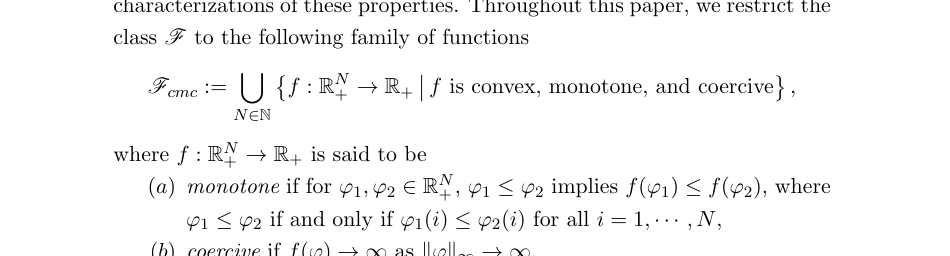
\includegraphics[width=.95\textwidth]{figures/function_class_crop.png}
\caption{The source definition of \(\Fc\).}
\end{figure}

Remark 3.12 asks:
\begin{quote}
``We do not know whether there exist two subspaces \(Y\) and \(Z\) of \(X\)
such that \((X,Y,\F(X))\) and \((X,Z,\F(X))\) has
\(\tau\)-\(\Fc\)-SACP, \(Y+Z\) is closed but \((X,Y+Z,\F(X))\) does not have
\(\tau\)-\(\Fc\)-SACP.''
\end{quote}

\begin{figure}[h]
\centering
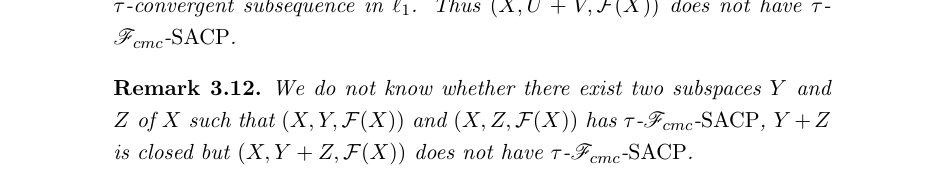
\includegraphics[width=.95\textwidth]{figures/open_remark_crop.png}
\caption{Remark 3.12 of \cite{Das2505}.}
\end{figure}

\section{The compactness forced by the plateau gauge}

\begin{lemma}\label{lem:ball}
Let \(V\) be a subspace of \(X\).
\begin{enumerate}
\item If \((X,V,\F(X))\) has norm-\(\Fc\)-SACP, then \(V\) is finite
dimensional.
\item If \((X,V,\F(X))\) has weak-\(\Fc\)-SACP, then \(V\) is reflexive.
\end{enumerate}
\end{lemma}

\begin{proof}
Let \(g:\mathbb R_+\to\mathbb R_+\) be
\[
g(t)=\max\{t-1,0\}.
\]
This \(g\) belongs to \(\Fc\): it is the maximum of two affine functions, hence
convex; it is increasing; and \(g(t)\to\infty\) as \(t\to\infty\).

Apply the SACP hypothesis to the one-point finite set \(F=\{0\}\).  Since
\(0\in V\),
\[
\rad_V^g(F)=\inf_{v\in V}g(\|v\|)=0.
\]
Moreover, for every \(v\in B_V\), \(g(\|v\|)=0\).  Hence every sequence in the
closed unit ball \(B_V\) is an exact minimizing sequence for \(g\) and \(F\).

If the topology is the norm topology, SACP says that every sequence in \(B_V\)
has a norm-convergent subsequence.  The norm topology is metric, so \(B_V\) is
norm compact.  By Riesz's lemma, the closed unit ball of a Banach space is norm
compact only in finite dimension.  Thus \(V\) is finite dimensional.

If the topology is the weak topology, SACP says that every sequence in \(B_V\)
has a weakly convergent subsequence in \(X\).  The set \(B_V\) is weakly closed
in \(X\), since \(V\) is a closed linear subspace and the unit ball is weakly
closed.  Thus \(B_V\) is weakly sequentially compact.  The weak topology on
\(V\) agrees with the topology inherited from the weak topology of \(X\), by
Hahn--Banach extension of functionals.  Eberlein--Smulian therefore implies
that \(B_V\) is weakly compact in \(V\).  Hence \(V\) is reflexive.
\end{proof}

\section{Answer to Remark 3.12}

\begin{theorem}\label{thm:main}
Let \(\tau\) be either the norm topology or the weak topology.  Let \(Y\) and
\(Z\) be subspaces of a Banach space \(X\) such that \(Y+Z\) is closed.  If
\((X,Y,\F(X))\) and \((X,Z,\F(X))\) both have \(\tau\)-\(\Fc\)-SACP, then
\((X,Y+Z,\F(X))\) has \(\tau\)-\(\Fc\)-SACP.
\end{theorem}

\begin{proof}
First suppose that \(\tau\) is the norm topology.  By Lemma
\ref{lem:ball}, \(Y\) is finite dimensional.  Theorem 3.10 of \cite{Das2505}
states that if \(Y\) is finite dimensional and \((X,Z,\F(X))\) has
\(\tau\)-\(\Fc\)-SACP, then \((X,Y+Z,\F(X))\) has \(\tau\)-\(\Fc\)-SACP.
This gives the conclusion.

Now suppose that \(\tau\) is the weak topology.  By Lemma \ref{lem:ball}, \(Y\)
is reflexive.  Theorem 3.14 of \cite{Das2505} states that if \(Y\) is a
reflexive subspace, \(Y+Z\) is closed, and \((X,Z,\F(X))\) has
weak-\(\Fc\)-SACP, then \((X,Y+Z,\F(X))\) has weak-\(\Fc\)-SACP.  This gives
the conclusion in the weak case.
\end{proof}

\begin{figure}[h]
\centering
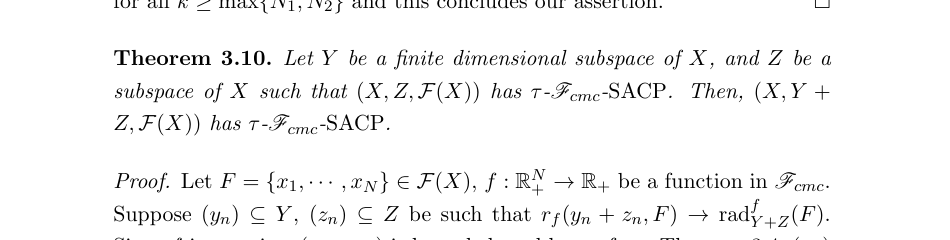
\includegraphics[width=.95\textwidth]{figures/finite_dim_transfer_crop.png}
\caption{The finite-dimensional transfer theorem, Theorem 3.10 of
\cite{Das2505}.}
\end{figure}

\begin{figure}[h]
\centering
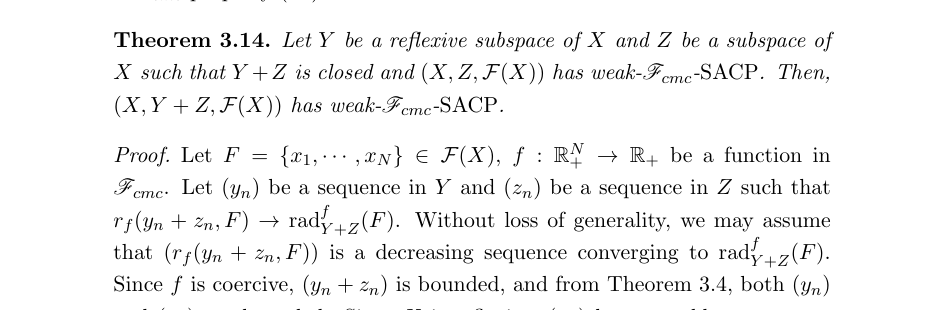
\includegraphics[width=.95\textwidth]{figures/weak_transfer_crop.png}
\caption{The weak/reflexive transfer theorem, Theorem 3.14 of \cite{Das2505}.}
\end{figure}

\begin{remark}
The proof uses the full function class \(\Fc\) exactly as defined in
\cite{Das2505}.  If one replaced \(\Fc\) by a narrower class, for example by
requiring strict increase or requiring the gauge to vanish only at the origin,
then the plateau-gauge argument would no longer apply.  That would be a
different question from Remark 3.12 as stated.
\end{remark}

\section{Novelty check}

The run's local indexes were searched for arXiv:2505.10851, the exact title,
the exact phrase from Remark 3.12, and the keywords \(\Fc\), SACP,
weak-\(\Fc\)-SACP, and \(Y+Z\).  No duplicate solution packet or
literature-answer packet was found.

External web/arXiv searches on 2026-06-19 for the exact remark phrase,
``Transfer of Approximation properties under Local Constraints Remark 3.12'',
``F\_cmc simultaneous approximative SACP subspaces'', and
``weak-F\_cmc-SACP reflexive subspace Y+Z'' found the source paper
\cite{Das2505} and the earlier SACP paper \cite{DasPaul2501}, but no later
paper explicitly answering this subspace-sum question.

\section{Human review recommendation}

This should be reviewed as a short claimed full solution.  The proof has only
one new observation, namely that the plateau gauge \(g(t)=\max\{t-1,0\}\) is
an allowed element of \(\Fc\) and converts the whole unit ball of a subspace
into exact minimizing sequences for \(F=\{0\}\).  Once that is accepted, the
source paper's Theorems 3.10 and 3.14 close the norm and weak cases.

\begin{thebibliography}{9}

\bibitem{Das2505}
Syamantak Das,
\emph{Transfer of Approximation properties under Local Constraints and Best
Simultaneous Approximation on Sums},
arXiv:2505.10851v3, 2026.
\url{https://arxiv.org/abs/2505.10851}

\bibitem{DasPaul2501}
Syamantak Das and Tanmoy Paul,
\emph{A study on \(\mathfrak F\)-simultaneous approximative
\(\tau\)-compactness property in Banach spaces},
arXiv:2501.03347, 2025.
\url{https://arxiv.org/abs/2501.03347}

\bibitem{Megginson}
Robert E. Megginson,
\emph{An Introduction to Banach Space Theory},
Graduate Texts in Mathematics 183, Springer, 1998.

\end{thebibliography}

\end{document}

